\chapter{L'authentification sur Stample}
\section*{}
\section{Introduction}
\paragraph{}
Dans une première partie suite à la tâche "Login sur Stample" assignée dans \textit{Trello}\footnote{https://trello.com/} avec Jonathan Winandy, j'ai commencé à lire, comprendre le code du backend Stample et à voir l'architecture du projet. 
\newline
\textit{Problématique, Comment faire pour intégrer une couche horizontal sans tout casser coté Frontend ?}
\subparagraph{}
Au début, j'ai implémenté une solution basique, relativement fonctionnel mais non achevé suite au complexités reliée à la compatibilité avec le code existant.
Ensuite, une deuxième approche en appliquant les méthodes d'ingénierie nous avons réussi à finaliser la tâche en moins de temps.

\subsection{Configuration du projet Stample}
\paragraph{}
J'ai eu l'accé au code source du projet privé sur le compte Git d'Edward avec son autorisation.
Au début, j'ai utilisé un outil windows pour la gestion de mes projets Git d'apprentissage.
Ensuite, j'ai changé mon PC parce que les outils SBT, play, mongo, ect... ont des besoins importants en ressources (mémoire,CPU). Stample m'a prêté un MacBookPro. 
\subparagraph{}
Pour interragir avec Stample, j'ai consolidé mes connaissances dans le terminal-land (tmux\footnote{http://tmux.sourceforge.net/}, zsh\footnote{https://github.com/robbyrussell/oh-my-zsh}, bash, git et SBT).
\section{Schema Model View Controller (MVC)}
\paragraph{}
Dans la plateforme Stample, les requêtes sont affectées aux controlleurs à l'aide de régles de routage. Les controlleurs utilisent des services et des repository du packges services/repository implémentés dans un sous package "impl" (implementation).
Les views contiennent les templates html.
C'est une architecture de play et généralement un design classique d'une application java que j'ai découvert.
\begin{figure}[H]
        \centering
                \centering
                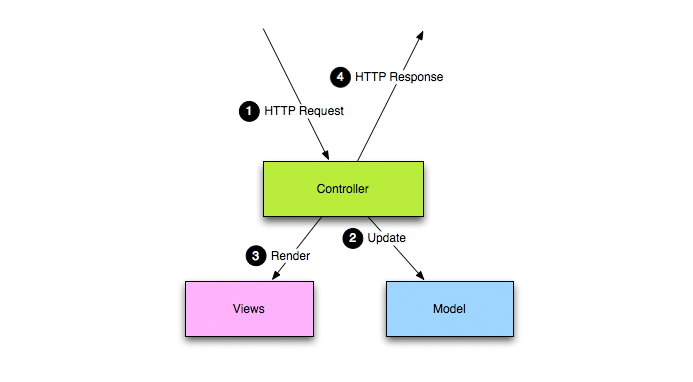
\includegraphics[width=\textwidth]{diagrams_mvc.png}
                \caption{Diagramme MVC}
                \label{fig:Diagramme MVC}
       
\end{figure}
\begin{itemize}
\item Model : Le modèle est la représentation spécifique au domaine de l'information sur laquelle l'application fonctionne. La logique de domaine ajoute «sens» aux données brutes (par exemple : le calcul des totaux, taxes de l'utilisateur, les frais d'expédition pour un panier, ect...). La plupart des applications utilisent un mécanisme de stockage persistant comme une base de données pour stocker des données. MVC ne mentionne pas spécifiquement la couche d'accès aux données, car il est entendu d'être en dessous, ou encapsulé par le modèle.
\item View : La vue rend le modèle dans une forme appropriée pour les interactions, en général une interface utilisateur. Plusieurs views peuvent exister pour un modèle unique, à des fins différentes. Dans un format de préférence "Web" (HTML, XML ou JSON) en fonction de la négociation avec le navigateur et des capacités du controlleur.
\item Controller : Le contrôleur répond aux événements (généralement des actions de l'utilisateur) et les traites, et peut également invoquer des changements sur le modèle. Dans une application Web, les événements sont généralement des requêtes HTTP: un contrôleur écoute les requêtes HTTP, extrait les données pertinentes de la «événement», telles que les paramètres de chaîne de requête, demander des têtes, ect... Et applique les modifications sur les objets du modèle sous-jacent.

\end{itemize}

\textit{Dans une application play ces trois couches sont définies dans un répertoire app, chacun dans un package,}
\begin{figure}[H]
        \centering
                \centering
                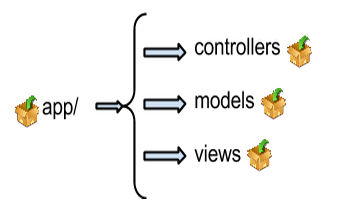
\includegraphics[width=\textwidth]{packages_play.png}
                \caption{Default play packages}
                \label{fig:Default play packages}
       
\end{figure}
\textit{Ainsi que d'aures packages qu'on a rajouté comme event, api, services, repository, plugins, templates, ect...}

\subsection{Cycle de vie d'une requête}
Le framework play est entièrement Stateless~\cite{rest} et orientée Request/Response. Tout les requête HTTP suivent le même path.
\begin{enumerate}
\item Une requête HTTP reçue par le framework.
\item Le Router Component essaie de trouver la route la plus spécifique en mesure d'accepter cette demande. Pour invoker la méthode d'action correspendante. 
\item Le code d'application est executée
\item Si une vue complexe doit être généré, un fichier template est rendu.
\item Le résultat de la méthode d'action (Code de réponse HTTP, Content) s'écrit alors comme une réponse HTTP.
\end{enumerate}
\begin{figure}[H]
        \centering
                \centering
                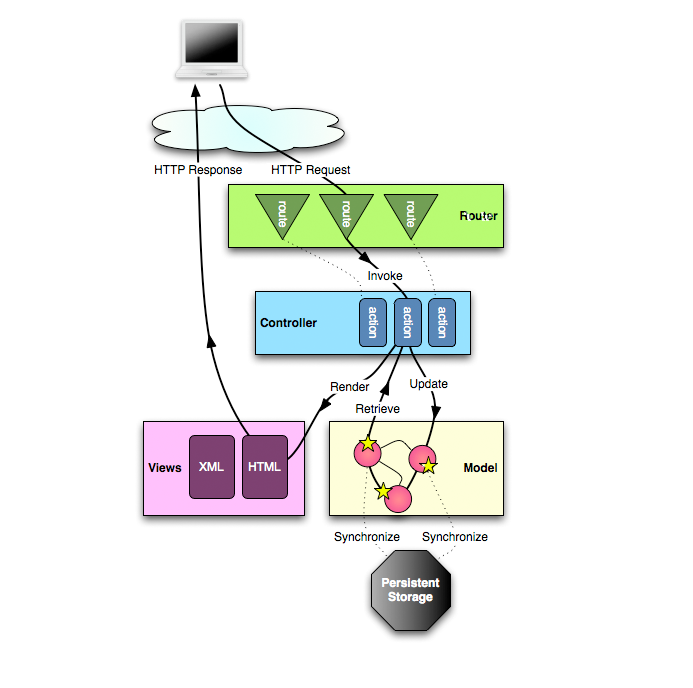
\includegraphics[width=\textwidth]{diagrams_path.png}
                \caption{Diagramme HTTP request path}
                \label{fig:Diagramme HTTP request path}
       
\end{figure}
\newpage
\section{Le login dans l'application existante}
\subsection{Login V0}
\paragraph{}
Dans la version précedente (version V0), il s'agit d'un formulaire classique à remplir pour créer un nouveau compte utilisateur qui sera stocker avec les coordonnées nécessaires (firstname, fullname, username, passeword, secretCode).
Cela est une première approche. Comme la plateforme est en cours de construction des nouveaux besoins apparaissent au fur et à mesure.
Pour plusieurs raisons : Satisfaire la clientèle (utilisateurs de Stample), faciliter la perception de l'interraction et offrir des nouvelles fonctionnalitées classique mais indisponsable.  
\subsection{Critiques}
\paragraph{}
Cette approche pour la gestion de la création d'un compte utilisateur sur Stample doit être refondues.
Il nous manque l'envoi des emails d'information lors des diffèrents étapes d'inscription notament le reset du mot de passe, ainsi que la possibilité de créer un compte à partir d'une autres plateformes en mesure que l'utilisateur s'ennui de reprendre tout un formulaire pour créer un nouveau compte sur une nouvelle plateforme.
\subsection{Fonctionalités manquantes}
\subsubsection{Envoi des mails}
\paragraph{}
Les utilisateurs de la platefome doivent être notifiés par email lors de l'inscription, l'activation du compte et le changement du mot de passe. 
Les diffèrents emails nécessaires sont signupEmail, welcomeEmail, alreadyRegistredEmail, unknownNotice, passwordResetEmail, passwordChangeNotice.
\subsubsection{Authentification avec d'autres plateformes}
\paragraph{}
Plusieurs sites web offrent à leurs utilisateurs la possibilité d'utiliser gmail, facebook, twitter ou autres pour le signup.
Cette fonctionnalités facilite l'inscription et rendre cette tâche rapide pour certains utilisateurs.
\subsubsection{Rest mot de passe}
\paragraph{}
Plusieurs utilisateurs, changent leurs mot de passe d'un site à un autre ce qui provoque souvent l'oublie du password.
La gestions des mots de passe oublié est parmi les fonctionnalités indispensable sur une plateforme.
\subsubsection{Activation code}
\paragraph{}
La version Beta de Stample est protégée avec un code d'activation, c'est une pratique habituelle pour sécuriser une plateforme mise en ligne et en cours de construction.
\section{Première approche}
\subsection{Etude du modéle}
\paragraph{}
Après quelques jours pour faire des considérations de conceptions et de mieux comprendre SecureSocial, j'ai réalisé que la mise en œuvre des méthodes n'était pas trop difficile à comprendre. C'est bien la conception de la logique dans un service backend qui compte. 
SecureSocial offre des APIs Scala et Java, on utilise ce module Scala pour le Backend de la plateforme.
Les services d'authentifications utilisent une catégorie des services de premiers plans comme Google, Twitter, Facebook ect..., Il offre aussi un mécanisme de username/password avec les fonctionnaliées Signup, Login, Rest Password.
\subparagraph{}
Ce module est compatible avec les versions de Play 2.1.x, 2.0.x et 1.x, les instructions pour l'intégration sur \textit{le site}\footnote{http://securesocial.ws/guide/getting-started.html}.
SecureSocial est extensible, il est basé sur un modèle de design qui vous permet d'ajouter des nouveaux services d'authentifications.

\subsection{Première Solution}
Les étapes d'implémentation: 
\begin{itemize}
\item J'ai ajouté une nouvelle table dans la base de donnée Stample pour mettre le hash (email, random number, time ),
\item Envoyer le mail avec un lien url?hash=\$hash,
\item Verifier d'existance du hash dans la base puis faire le tri.

\end{itemize}
Solution que j'ai envisagé, elle a provoqué une approche non stable en terme d'efficacité et de consistance.
\section{Deuxième approche}
\subsection{Phase préliminaire}
D'après Jonathan Winandy, pour réussir il faut passer par les étapes suivantes :
\begin{itemize}

\item Do It :Commencer par poser le problème et puis écrire du code qui répond à ce besoin.  
\item Do It-Right : Se débarrasser du code inutile, faire des testes et des amélioration.
\item Do It-Fast : Nettoyer le code et vérifier les tests.
\end{itemize}

\subsection{Sauvegarde de session}
\paragraph{}
Dans le fichier de configuration de SecureSocial, J'avais besoin de changer : La configuration des cookies "absoluteTimeOutInMinutes"(La durée d'authentification d'un utilisateur dans une session), l'utilisateur doit relogger après ce timing de 720 minutes (par défaut) à 7200 minutes.
La durée de session valable depuis la dernière requête  "idleTimeoutInMinutes" de 30 minutes (par défaut) à 42000 minutes.
Comme le sujet, l'idée est de limiter les partie amovible, donc on s'est simuler une implimentation "in-memory" de l'authentificaion pour commencer.
\subsection{Customisation des templates}
\paragraph{}
Après l'intégration et la stabilisation des différentes interractions avec le module, j'ai travaillé pour refactoriser les différentes views pour s'adapter avec ce module (le signup, resetPasswordPage, authorisationCode, startResetPassword) et un main global.
L'activationCode c'est un code secret pour protéger la version Beta de Stample(autoriser l'accé qu'à certain utilisateur), il y avait un activationCode écrit dans le code de la plateforme que nous avons enlevé pour mettre dans l'interface admin la possibilité de génèrer des diffirents codes d'autorisations.
\section{Implémentation \& Intégration}
Pour l'intégration de SecureSocial 
\[
Do It =
\begin{cases}
\text{La vérification de compilation, intégration basique de secure Social dans Stample.}\\
\text{Une écriture basique dans la mémoire et l'implémentation de UserService.}\\
\text{Working Wiring : Authentification avec email.}
\end{cases}
\]
\[
Do It-Righ =
\begin{cases}
\text{Ajout du template signUp email.}\\
\text{Résoudre les problèmes de Token et de Memory.}
\end{cases}
\]
\textit{L'étape Do It-Fast n'est pas encore faite mais elle pourrait être mise dans le planing des tâches plus tard. }
\section{Partie Administrateur sur Stample}
\paragraph{}
Stample c'est un réseau social en cours de construction il y avait plusieurs bugs et amélioration à ajouter sur la plateforme durant mon stage.
Parmis ces amélioration l'ajout dans l'interface administrateur de l'API la possibilité de génerer/écrire un code
secret pour les utilisateurs lors de l'inscription avec un nombre d'usage pour chaque code.
Cela nécessite l'ajout des routes pour gérer et créer les codes d'authentification dans l'admin 
controller et les templates.
J'ai implémenté les différentes templates (authorisationCodes, createCode).
\begin{figure}[H]
\begin{minipage}[c]{.5\linewidth}
\begin{center}
\fbox{
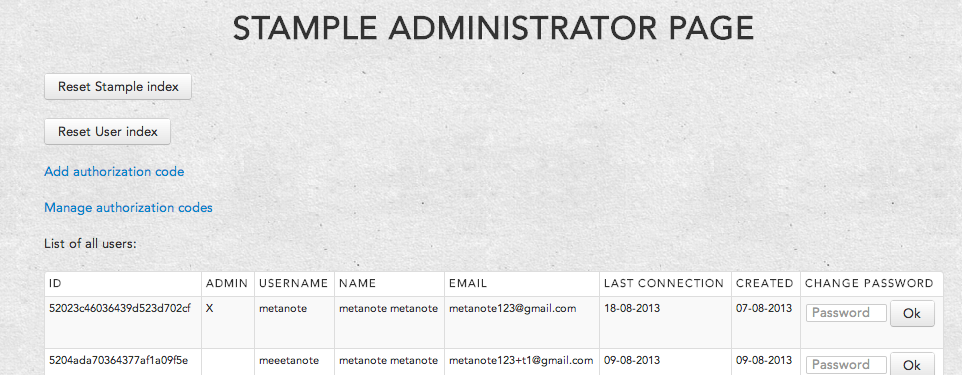
\includegraphics[width=5.5cm,height=80mm,scale=1]{image2.png}}
\caption{Admin page}
\label{fig:Admin page}
\end{center}
\end{minipage}
\hfill
\begin{minipage}[c]{.5\linewidth}
\begin{center}
\fbox{
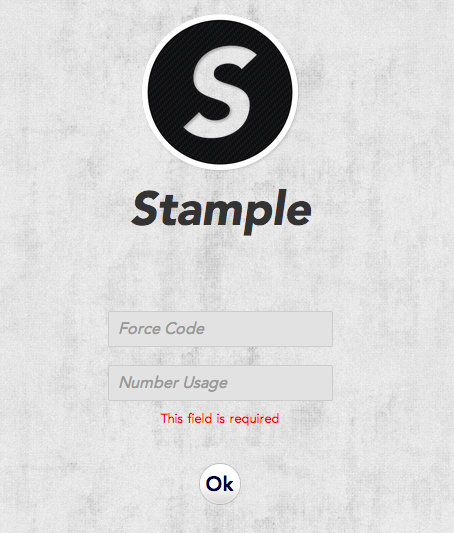
\includegraphics[width=5.5cm,height=80mm,scale=1]{image1.png}}\hspace{1em}
\caption{Create secret interface}
\label{fig:Create authorisationCode interface}
\end{center}
\end{minipage}
\end{figure}
\textit{Depuis l'interface Admin le bouton create add autorization code ouvre la deuxième interface pour la creation d'un code secret aléatoire avec un le nombre d'usage qui est un champ obligatoire ou bien en choisissant un code d'autorisation.
Le bouton manage authorisation codes permet d'afficher les codes d'authorisation enregistrer et le nombre d'usage restant.
}
\section{Résumé}
\paragraph{}
Cette partie d'authentification sur Stample m'a beaucoup apporté en écrivant du code/des templates et en fixant des bugs.
Sur Backend, l'interaction des controllers, les models et les views avec les différentes classes et traits existant m'avait permis de comprendre le langage en ajoutant du code compatible.
\subparagraph{}
Cette partie du développement m'a permis de reconnaitre le plugin SecureSocial qui peut servir dans d'autres projets et d'améliorer mes connaissances. 
Ce plugin sera peut-être enlevé, remplacé plus tard par l'authentification avec WebID. 
